
\begin{DoxyItemize}
\item \hyperlink{random_rand}{R\-A\-N\-D Uniform Random Number Generator}  
\item \hyperlink{random_randbeta}{R\-A\-N\-D\-B\-E\-T\-A Beta Deviate Random Number Generator}  
\item \hyperlink{random_randbin}{R\-A\-N\-D\-B\-I\-N Generate Binomial Random Variables}  
\item \hyperlink{random_randchi}{R\-A\-N\-D\-C\-H\-I Generate Chi-\/\-Square Random Variable}  
\item \hyperlink{random_randexp}{R\-A\-N\-D\-E\-X\-P Generate Exponential Random Variable}  
\item \hyperlink{random_randf}{R\-A\-N\-D\-F Generate F-\/\-Distributed Random Variable}  
\item \hyperlink{random_randgamma}{R\-A\-N\-D\-G\-A\-M\-M\-A Generate Gamma-\/\-Distributed Random Variable}  
\item \hyperlink{random_randi}{R\-A\-N\-D\-I Uniformly Distributed Integer}  
\item \hyperlink{random_randmulti}{R\-A\-N\-D\-M\-U\-L\-T\-I Generate Multinomial-\/distributed Random Variables}  
\item \hyperlink{random_randn}{R\-A\-N\-D\-N Gaussian (Normal) Random Number Generator}  
\item \hyperlink{random_randnbin}{R\-A\-N\-D\-N\-B\-I\-N Generate Negative Binomial Random Variables}  
\item \hyperlink{random_randnchi}{R\-A\-N\-D\-N\-C\-H\-I Generate Noncentral Chi-\/\-Square Random Variable}  
\item \hyperlink{random_randnf}{R\-A\-N\-D\-N\-F Generate Noncentral F-\/\-Distribution Random Variable}  
\item \hyperlink{random_randp}{R\-A\-N\-D\-P Generate Poisson Random Variable}  
\item \hyperlink{random_randperm}{R\-A\-N\-D\-P\-E\-R\-M Random permutation}  
\item \hyperlink{random_seed}{S\-E\-E\-D Seed the Random Number Generator}  
\end{DoxyItemize}\hypertarget{random_rand}{}\section{R\-A\-N\-D Uniform Random Number Generator}\label{random_rand}
Section\-: \hyperlink{sec_random}{Random Number Generation} \hypertarget{vtkwidgets_vtkxyplotwidget_Usage}{}\subsection{Usage}\label{vtkwidgets_vtkxyplotwidget_Usage}
Creates an array of pseudo-\/random numbers of the specified size. The numbers are uniformly distributed on {\ttfamily \mbox{[}0,1)}. Two seperate syntaxes are possible. The first syntax specifies the array dimensions as a sequence of scalar dimensions\-: \begin{DoxyVerb}  y = rand(d1,d2,...,dn).
\end{DoxyVerb}
 The resulting array has the given dimensions, and is filled with random numbers. The type of {\ttfamily y} is {\ttfamily double}, a 64-\/bit floating point array. To get arrays of other types, use the typecast functions.

The second syntax specifies the array dimensions as a vector, where each element in the vector specifies a dimension length\-: \begin{DoxyVerb}  y = rand([d1,d2,...,dn]).
\end{DoxyVerb}
 This syntax is more convenient for calling {\ttfamily rand} using a variable for the argument.

Finally, {\ttfamily rand} supports two additional forms that allow you to manipulate the state of the random number generator. The first retrieves the state \begin{DoxyVerb}  y = rand('state')
\end{DoxyVerb}
 which is a 625 length integer vector. The second form sets the state \begin{DoxyVerb}  rand('state',y)
\end{DoxyVerb}
 or alternately, you can reset the random number generator with \begin{DoxyVerb}  rand('state',0)
\end{DoxyVerb}
 \hypertarget{variables_struct_Example}{}\subsection{Example}\label{variables_struct_Example}
The following example demonstrates an example of using the first form of the {\ttfamily rand} function.


\begin{DoxyVerbInclude}
--> rand(2,2,2)

ans = 

(:,:,1) = 
    0.8539    0.1733 
    0.0415    0.1300 

(:,:,2) = 
    0.7163    0.5752 
    0.5953    0.3728 
\end{DoxyVerbInclude}


The second example demonstrates the second form of the {\ttfamily rand} function.


\begin{DoxyVerbInclude}
--> rand([2,2,2])

ans = 

(:,:,1) = 
    0.4992    0.2797 
    0.6513    0.3209 

(:,:,2) = 
    0.6244    0.7774 
    0.0934    0.1820 
\end{DoxyVerbInclude}


The third example computes the mean and variance of a large number of uniform random numbers. Recall that the mean should be {\ttfamily 1/2}, and the variance should be {\ttfamily 1/12 $\sim$ 0.\-083}.


\begin{DoxyVerbInclude}
--> x = rand(1,10000);
--> mean(x)

ans = 
    0.4952 

--> var(x)

ans = 
    0.0845 
\end{DoxyVerbInclude}


Now, we use the state manipulation functions of {\ttfamily rand} to exactly reproduce a random sequence. Note that unlike using {\ttfamily seed}, we can exactly control where the random number generator starts by saving the state.


\begin{DoxyVerbInclude}
--> rand('state',0)    % restores us to startup conditions
--> a = rand(1,3)      % random sequence 1

a = 
    0.3759    0.0183    0.9134 

--> b = rand('state'); % capture the state vector
--> c = rand(1,3)      % random sequence 2  

c = 
    0.3580    0.7604    0.8077 

--> rand('state',b);   % restart the random generator so...
--> c = rand(1,3)      % we get random sequence 2 again

c = 
    0.3580    0.7604    0.8077 
\end{DoxyVerbInclude}
 \hypertarget{random_randbeta}{}\section{R\-A\-N\-D\-B\-E\-T\-A Beta Deviate Random Number Generator}\label{random_randbeta}
Section\-: \hyperlink{sec_random}{Random Number Generation} \hypertarget{vtkwidgets_vtkxyplotwidget_Usage}{}\subsection{Usage}\label{vtkwidgets_vtkxyplotwidget_Usage}
Creates an array of beta random deviates based on the supplied two parameters. The general syntax for {\ttfamily randbeta} is \begin{DoxyVerb}   y = randbeta(alpha, beta)
\end{DoxyVerb}
 where {\ttfamily alpha} and {\ttfamily beta} are the two parameters of the random deviate. There are three forms for calling {\ttfamily randbeta}. The first uses two vectors {\ttfamily alpha} and {\ttfamily beta} of the same size, in which case the output {\ttfamily y} is the same size as both inputs, and each deviate uses the corresponding values of {\ttfamily alpha} and {\ttfamily beta} from the arguments. In the other forms, either {\ttfamily alpha} or {\ttfamily beta} are scalars. \hypertarget{transforms_svd_Function}{}\subsection{Internals}\label{transforms_svd_Function}
The probability density function (P\-D\-F) of a beta random variable is \[ f(x) = x^(a-1) * (1-x)^(b-1) / B(a,b) \] for {\ttfamily x} between 0 and 1. The function {\ttfamily B(a,b)} is defined so that the integral of {\ttfamily f(x)} is 1. \hypertarget{variables_struct_Example}{}\subsection{Example}\label{variables_struct_Example}
Here is a plot of the P\-D\-F of a beta random variable with {\ttfamily a=3}, {\ttfamily b=7}.


\begin{DoxyVerbInclude}
--> a = 3; b = 7;
--> x = (0:100)/100; t = x.^(a-1).*(1-x).^(b-1); 
--> t = t/(sum(t)*.01);
--> plot(x,t);
\end{DoxyVerbInclude}


which is plotted as  
\begin{DoxyImage}
\includegraphics[width=12cm]{betapdf}
\caption{betapdf}
\end{DoxyImage}
 If we generate a few random deviates with these values, we see they are distributed around the peak of roughly {\ttfamily 0.\-25}.


\begin{DoxyVerbInclude}
--> randbeta(3*ones(1,5),7*ones(1,5))

ans = 
    0.4343    0.4220    0.3992    0.2727    0.2475 
\end{DoxyVerbInclude}
 \hypertarget{random_randbin}{}\section{R\-A\-N\-D\-B\-I\-N Generate Binomial Random Variables}\label{random_randbin}
Section\-: \hyperlink{sec_random}{Random Number Generation} \hypertarget{vtkwidgets_vtkxyplotwidget_Usage}{}\subsection{Usage}\label{vtkwidgets_vtkxyplotwidget_Usage}
Generates random variables with a binomial distribution. The general syntax for its use is \begin{DoxyVerb}   y = randbin(N,p)
\end{DoxyVerb}
 where {\ttfamily N} is a vector representing the number of Bernoulli trials, and {\ttfamily p} is the success probability associated with each trial. \hypertarget{transforms_svd_Function}{}\subsection{Internals}\label{transforms_svd_Function}
A Binomial random variable describes the number of successful outcomes from {\ttfamily N} Bernoulli trials, with the probability of success in each trial being {\ttfamily p}. The probability distribution is \[ P(n) = \frac{N!}{n!(N-n)!}p^n(1-p)^{N-n} \] \hypertarget{variables_struct_Example}{}\subsection{Example}\label{variables_struct_Example}
Here we generate {\ttfamily 10} binomial random variables, corresponding to {\ttfamily N=100} trials, each with probability {\ttfamily p=0.\-1}, using both {\ttfamily randbin} and then again using {\ttfamily rand} (to simulate the trials)\-:


\begin{DoxyVerbInclude}
--> randbin(100,.1*ones(1,10))

ans = 
  6  7  6  7 13  7  7 10 13 15 

--> sum(rand(100,10)<0.1)

ans = 
 11  9  8  9 15 16 11 17  4  7 
\end{DoxyVerbInclude}
 \hypertarget{random_randchi}{}\section{R\-A\-N\-D\-C\-H\-I Generate Chi-\/\-Square Random Variable}\label{random_randchi}
Section\-: \hyperlink{sec_random}{Random Number Generation} \hypertarget{vtkwidgets_vtkxyplotwidget_Usage}{}\subsection{Usage}\label{vtkwidgets_vtkxyplotwidget_Usage}
Generates a vector of chi-\/square random variables with the given number of degrees of freedom. The general syntax for its use is \begin{DoxyVerb}   y = randchi(n)
\end{DoxyVerb}
 where {\ttfamily n} is an array containing the degrees of freedom for each generated random variable. \hypertarget{transforms_svd_Function}{}\subsection{Internals}\label{transforms_svd_Function}
A chi-\/square random variable is essentially distributed as the squared Euclidean norm of a vector of standard Gaussian random variables. The number of degrees of freedom is generally the number of elements in the vector. In general, the P\-D\-F of a chi-\/square random variable is \[ f(x) = \frac{x^{r/2-1}e^{-x/2}}{\Gamma(r/2)2^{r/2}} \] \hypertarget{variables_struct_Example}{}\subsection{Example}\label{variables_struct_Example}
First, a plot of the P\-D\-F for a family of chi-\/square random variables


\begin{DoxyVerbInclude}
--> f = zeros(7,100);
--> x = (1:100)/10;
--> for n=1:7;t=x.^(n/2-1).*exp(-x/2);f(n,:)=10*t/sum(t);end
--> plot(x,f');
\end{DoxyVerbInclude}


The P\-D\-F is below\-:  
\begin{DoxyImage}
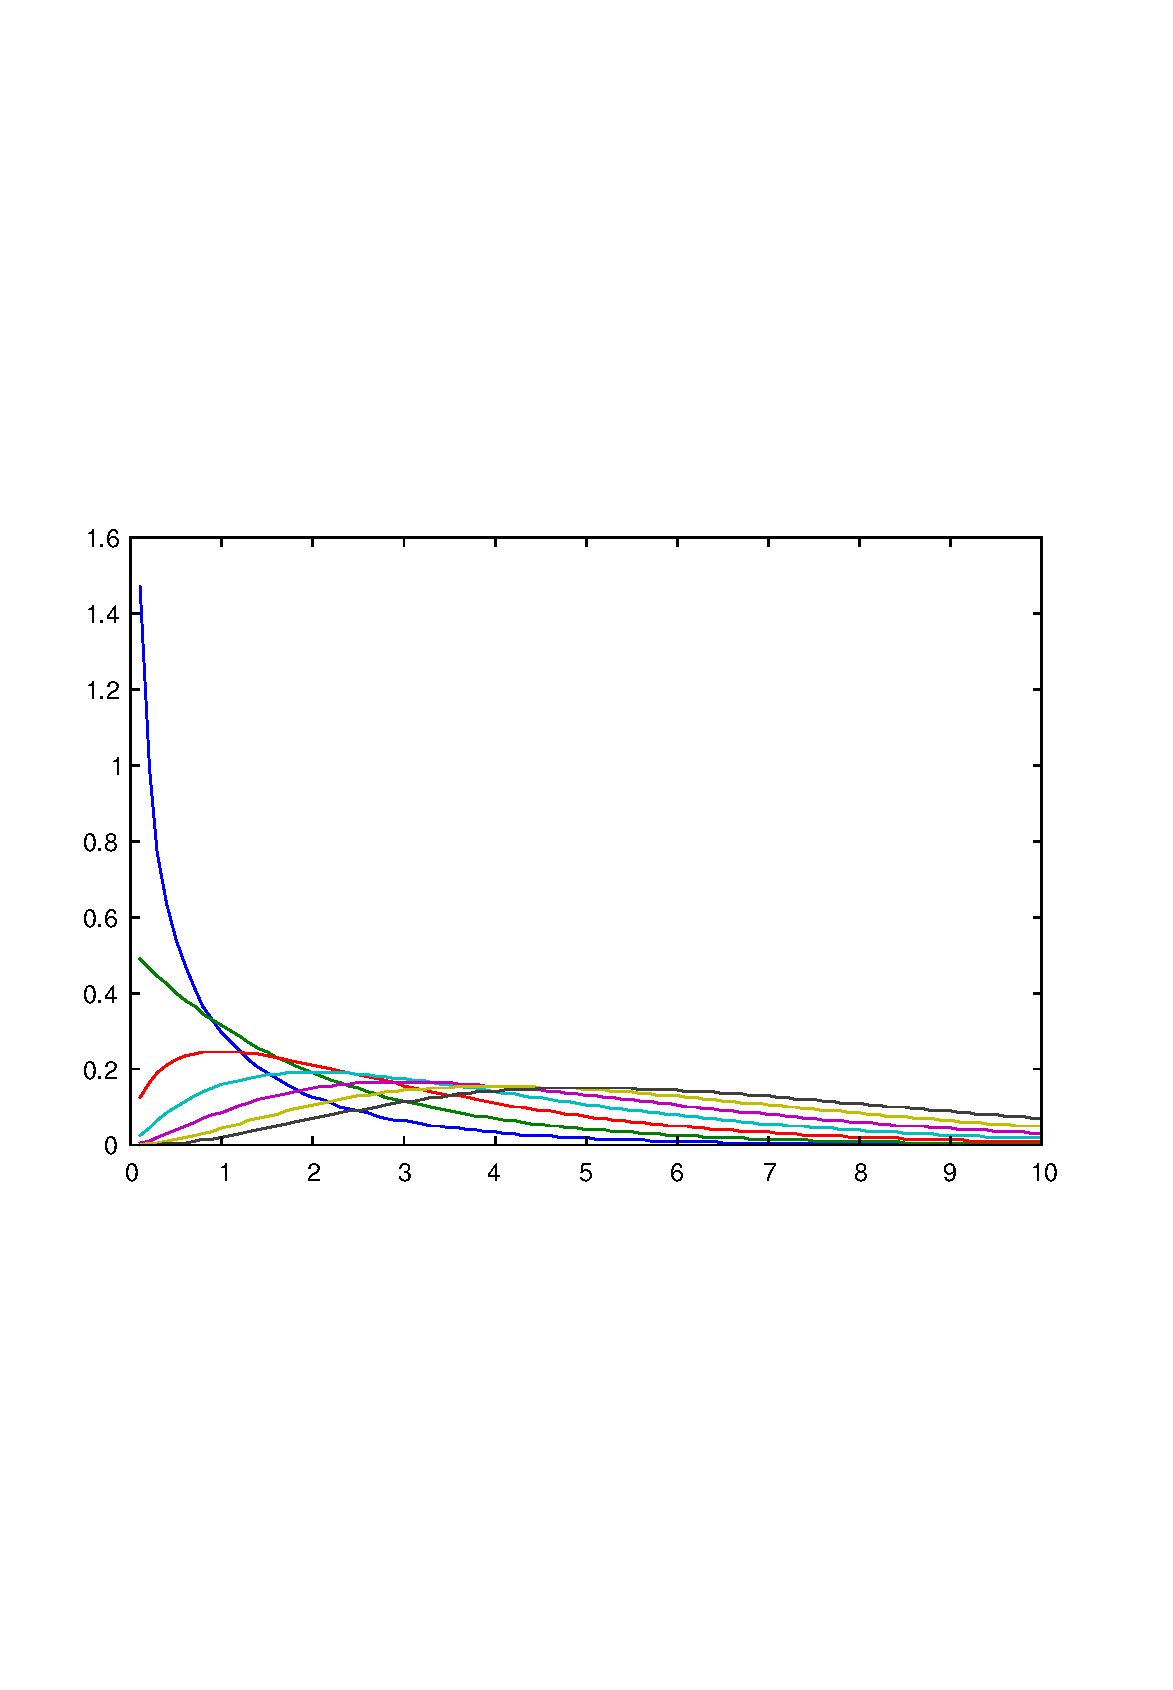
\includegraphics[width=12cm]{chipdf}
\caption{chipdf}
\end{DoxyImage}
 Here is an example of using {\ttfamily randchi} and {\ttfamily randn} to compute some chi-\/square random variables with four degrees of freedom.


\begin{DoxyVerbInclude}
--> randchi(4*ones(1,6))

ans = 
    2.6122    6.2362    0.8717    1.4935    6.0370    5.2771 

--> sum(randn(4,6).^2)

ans = 
    0.0399    4.6296    0.8697    0.5796    1.5490    5.8538 
\end{DoxyVerbInclude}
 \hypertarget{random_randexp}{}\section{R\-A\-N\-D\-E\-X\-P Generate Exponential Random Variable}\label{random_randexp}
Section\-: \hyperlink{sec_random}{Random Number Generation} \hypertarget{vtkwidgets_vtkxyplotwidget_Usage}{}\subsection{Usage}\label{vtkwidgets_vtkxyplotwidget_Usage}
Generates a vector of exponential random variables with the specified parameter. The general syntax for its use is \begin{DoxyVerb}   y = randexp(lambda)
\end{DoxyVerb}
 where {\ttfamily lambda} is a vector containing the parameters for the generated random variables. \hypertarget{transforms_svd_Function}{}\subsection{Internals}\label{transforms_svd_Function}
The exponential random variable is usually associated with the waiting time between events in a Poisson random process. The P\-D\-F of an exponential random variable is\-: \[ f(x) = \lambda e^{-\lambda x} \] \hypertarget{variables_struct_Example}{}\subsection{Example}\label{variables_struct_Example}
Here is an example of using the {\ttfamily randexp} function to generate some exponentially distributed random variables


\begin{DoxyVerbInclude}
--> randexp(ones(1,6))

ans = 
    0.7969    0.2401    0.5891    1.5129    0.9998    2.7738 
\end{DoxyVerbInclude}
 \hypertarget{random_randf}{}\section{R\-A\-N\-D\-F Generate F-\/\-Distributed Random Variable}\label{random_randf}
Section\-: \hyperlink{sec_random}{Random Number Generation} \hypertarget{vtkwidgets_vtkxyplotwidget_Usage}{}\subsection{Usage}\label{vtkwidgets_vtkxyplotwidget_Usage}
Generates random variables with an F-\/distribution. The general syntax for its use is \begin{DoxyVerb}   y = randf(n,m)
\end{DoxyVerb}
 where {\ttfamily n} and {\ttfamily m} are vectors of the number of degrees of freedom in the numerator and denominator of the chi-\/square random variables whose ratio defines the statistic. \hypertarget{transforms_svd_Function}{}\subsection{Internals}\label{transforms_svd_Function}
The statistic {\ttfamily F\-\_\-\{n,m\}} is defined as the ratio of two chi-\/square random variables\-: \[ F_{n,m} = \frac{\chi_n^2/n}{\chi_m^2/m} \] The P\-D\-F is given by \[ f_{n,m} = \frac{m^{m/2}n^{n/2}x^{n/2-1}}{(m+nx)^{(n+m)/2}B(n/2,m/2)}, \] where {\ttfamily B(a,b)} is the beta function. \hypertarget{variables_struct_Example}{}\subsection{Example}\label{variables_struct_Example}
Here we use {\ttfamily randf} to generate some F-\/distributed random variables, and then again using the {\ttfamily randchi} function\-:


\begin{DoxyVerbInclude}
--> randf(5*ones(1,9),7)

ans = 

 Columns 1 to 7

    0.5241    0.8414    0.4859    1.1266    0.4792    2.3743    2.9095 

 Columns 8 to 9

    0.5825    0.4244 

--> randchi(5*ones(1,9))./randchi(7*ones(1,9))

ans = 

 Columns 1 to 7

    0.3737    0.2363    1.5733    0.7003    1.1385    0.6337    0.4597 

 Columns 8 to 9

    0.2691    0.5190 
\end{DoxyVerbInclude}
 \hypertarget{random_randgamma}{}\section{R\-A\-N\-D\-G\-A\-M\-M\-A Generate Gamma-\/\-Distributed Random Variable}\label{random_randgamma}
Section\-: \hyperlink{sec_random}{Random Number Generation} \hypertarget{vtkwidgets_vtkxyplotwidget_Usage}{}\subsection{Usage}\label{vtkwidgets_vtkxyplotwidget_Usage}
Generates random variables with a gamma distribution. The general syntax for its use is \begin{DoxyVerb}   y = randgamma(a,r),
\end{DoxyVerb}
 where {\ttfamily a} and {\ttfamily r} are vectors describing the parameters of the gamma distribution. Roughly speaking, if {\ttfamily a} is the mean time between changes of a Poisson random process, and we wait for the {\ttfamily r} change, the resulting wait time is Gamma distributed with parameters {\ttfamily a} and {\ttfamily r}. \hypertarget{transforms_svd_Function}{}\subsection{Internals}\label{transforms_svd_Function}
The Gamma distribution arises in Poisson random processes. It represents the waiting time to the occurance of the {\ttfamily r}-\/th event in a process with mean time {\ttfamily a} between events. The probability distribution of a Gamma random variable is \[ P(x) = \frac{a^r x^{r-1} e^{-ax}}{\Gamma(r)}. \] Note also that for integer values of {\ttfamily r} that a Gamma random variable is effectively the sum of {\ttfamily r} exponential random variables with parameter {\ttfamily a}. \hypertarget{variables_struct_Example}{}\subsection{Example}\label{variables_struct_Example}
Here we use the {\ttfamily randgamma} function to generate Gamma-\/distributed random variables, and then generate them again using the {\ttfamily randexp} function.


\begin{DoxyVerbInclude}
--> randgamma(1,15*ones(1,9))

ans = 

 Columns 1 to 7

   10.0227   12.4783   18.0388   21.7056   14.1249   15.9260   22.0177 

 Columns 8 to 9

   15.9170   24.3781 

--> sum(randexp(ones(15,9)))

ans = 

 Columns 1 to 7

   14.5031   12.8908   10.5201   16.9976    9.8463   12.7479   13.6879 

 Columns 8 to 9

   21.7005   11.4172 
\end{DoxyVerbInclude}
 \hypertarget{random_randi}{}\section{R\-A\-N\-D\-I Uniformly Distributed Integer}\label{random_randi}
Section\-: \hyperlink{sec_random}{Random Number Generation} \hypertarget{vtkwidgets_vtkxyplotwidget_Usage}{}\subsection{Usage}\label{vtkwidgets_vtkxyplotwidget_Usage}
Generates an array of uniformly distributed integers between the two supplied limits. The general syntax for {\ttfamily randi} is \begin{DoxyVerb}   y = randi(low,high)
\end{DoxyVerb}
 where {\ttfamily low} and {\ttfamily high} are arrays of integers. Scalars can be used for one of the arguments. The output {\ttfamily y} is a uniformly distributed pseudo-\/random number between {\ttfamily low} and {\ttfamily high} (inclusive). \hypertarget{variables_struct_Example}{}\subsection{Example}\label{variables_struct_Example}
Here is an example of a set of random integers between zero and 5\-:


\begin{DoxyVerbInclude}
--> randi(zeros(1,6),5*ones(1,6))

ans = 
 5 5 0 4 4 2 
\end{DoxyVerbInclude}
 \hypertarget{random_randmulti}{}\section{R\-A\-N\-D\-M\-U\-L\-T\-I Generate Multinomial-\/distributed Random Variables}\label{random_randmulti}
Section\-: \hyperlink{sec_random}{Random Number Generation} \hypertarget{vtkwidgets_vtkxyplotwidget_Usage}{}\subsection{Usage}\label{vtkwidgets_vtkxyplotwidget_Usage}
This function generates samples from a multinomial distribution given the probability of each outcome. The general syntax for its use is \begin{DoxyVerb}   y = randmulti(N,pvec)
\end{DoxyVerb}
 where {\ttfamily N} is the number of experiments to perform, and {\ttfamily pvec} is the vector of probabilities describing the distribution of outcomes. \hypertarget{transforms_svd_Function}{}\subsection{Internals}\label{transforms_svd_Function}
A multinomial distribution describes the number of times each of {\ttfamily m} possible outcomes occurs out of {\ttfamily N} trials, where each outcome has a probability {\ttfamily p\-\_\-i}. More generally, suppose that the probability of a Bernoulli random variable {\ttfamily X\-\_\-i} is {\ttfamily p\-\_\-i}, and that \[ \sum_{i=1}^{m} p_i = 1. \] Then the probability that {\ttfamily X\-\_\-i} occurs {\ttfamily x\-\_\-i} times is \[ P_N(x_1,x_2,\ldots,x_n) = \frac{N!}{x_1!\cdots x_n!} p_1^{x_1}\cdots p_n^{x_n}. \] \hypertarget{variables_struct_Example}{}\subsection{Example}\label{variables_struct_Example}
Suppose an experiment has three possible outcomes, say heads, tails and edge, with probabilities {\ttfamily 0.\-4999}, {\ttfamily 0.\-4999} and {\ttfamily 0.\-0002}, respectively. Then if we perform ten thousand coin flips we get


\begin{DoxyVerbInclude}
--> randmulti(10000,[0.4999,0.4999,0.0002])

ans = 
 5051    0 4948 
\end{DoxyVerbInclude}
 \hypertarget{random_randn}{}\section{R\-A\-N\-D\-N Gaussian (Normal) Random Number Generator}\label{random_randn}
Section\-: \hyperlink{sec_random}{Random Number Generation} \hypertarget{vtkwidgets_vtkxyplotwidget_Usage}{}\subsection{Usage}\label{vtkwidgets_vtkxyplotwidget_Usage}
Creates an array of pseudo-\/random numbers of the specified size. The numbers are normally distributed with zero mean and a unit standard deviation (i.\-e., {\ttfamily mu = 0, sigma = 1}). Two seperate syntaxes are possible. The first syntax specifies the array dimensions as a sequence of scalar dimensions\-: \begin{DoxyVerb}  y = randn(d1,d2,...,dn).
\end{DoxyVerb}
 The resulting array has the given dimensions, and is filled with random numbers. The type of {\ttfamily y} is {\ttfamily double}, a 64-\/bit floating point array. To get arrays of other types, use the typecast functions.

The second syntax specifies the array dimensions as a vector, where each element in the vector specifies a dimension length\-: \begin{DoxyVerb}  y = randn([d1,d2,...,dn]).
\end{DoxyVerb}
 This syntax is more convenient for calling {\ttfamily randn} using a variable for the argument.

Finally, {\ttfamily randn} supports two additional forms that allow you to manipulate the state of the random number generator. The first retrieves the state \begin{DoxyVerb}  y = randn('state')
\end{DoxyVerb}
 which is a 625 length integer vector. The second form sets the state \begin{DoxyVerb}  randn('state',y)
\end{DoxyVerb}
 or alternately, you can reset the random number generator with \begin{DoxyVerb}  randn('state',0)
\end{DoxyVerb}
 \hypertarget{transforms_svd_Function}{}\subsection{Internals}\label{transforms_svd_Function}
Recall that the probability density function (P\-D\-F) of a normal random variable is \[ f(x) = \frac{1}{\sqrt{2\pi \sigma^2}} e^{\frac{-(x-\mu)^2}{2\sigma^2}}. \] The Gaussian random numbers are generated from pairs of uniform random numbers using a transformation technique. \hypertarget{variables_struct_Example}{}\subsection{Example}\label{variables_struct_Example}
The following example demonstrates an example of using the first form of the {\ttfamily randn} function.


\begin{DoxyVerbInclude}
--> randn(2,2,2)

ans = 

(:,:,1) = 
   -1.3838    0.9091 
   -1.1738    0.1705 

(:,:,2) = 
   -0.0336    0.4572 
    0.7566   -1.1720 
\end{DoxyVerbInclude}


The second example demonstrates the second form of the {\ttfamily randn} function.


\begin{DoxyVerbInclude}
--> randn([2,2,2])

ans = 

(:,:,1) = 
    1.2183   -0.5558 
    0.1605    0.1819 

(:,:,2) = 
    0.5727   -0.5929 
   -0.3895   -0.2424 
\end{DoxyVerbInclude}


In the next example, we create a large array of 10000 normally distributed pseudo-\/random numbers. We then shift the mean to 10, and the variance to 5. We then numerically calculate the mean and variance using {\ttfamily mean} and {\ttfamily var}, respectively.


\begin{DoxyVerbInclude}
--> x = 10+sqrt(5)*randn(1,10000);
--> mean(x)

ans = 
   10.0370 

--> var(x)

ans = 
    4.9402 
\end{DoxyVerbInclude}


Now, we use the state manipulation functions of {\ttfamily randn} to exactly reproduce a random sequence. Note that unlike using {\ttfamily seed}, we can exactly control where the random number generator starts by saving the state.


\begin{DoxyVerbInclude}
--> randn('state',0)    % restores us to startup conditions
--> a = randn(1,3)      % random sequence 1

a = 
   -0.0362   -0.1404    0.6934 

--> b = randn('state'); % capture the state vector
--> c = randn(1,3)      % random sequence 2  

c = 
    0.5998    0.7086   -0.9394 

--> randn('state',b);   % restart the random generator so...
--> c = randn(1,3)      % we get random sequence 2 again

c = 
    0.5998    0.7086   -0.9394 
\end{DoxyVerbInclude}
 \hypertarget{random_randnbin}{}\section{R\-A\-N\-D\-N\-B\-I\-N Generate Negative Binomial Random Variables}\label{random_randnbin}
Section\-: \hyperlink{sec_random}{Random Number Generation} \hypertarget{vtkwidgets_vtkxyplotwidget_Usage}{}\subsection{Usage}\label{vtkwidgets_vtkxyplotwidget_Usage}
Generates random variables with a negative binomial distribution. The general syntax for its use is \begin{DoxyVerb}   y = randnbin(r,p)
\end{DoxyVerb}
 where {\ttfamily r} is a vector of integers representing the number of successes, and {\ttfamily p} is the probability of success. \hypertarget{transforms_svd_Function}{}\subsection{Internals}\label{transforms_svd_Function}
A negative binomial random variable describes the number of failures {\ttfamily x} that occur in {\ttfamily x+r} bernoulli trials, with a success on the {\ttfamily x+r} trial. The pdf is given by \[ P_{r,p}(x)=\left(\begin{matrix} x+r-1 \\ r-1 \end{matrix}\right)p^r(1-p)^x. \] \hypertarget{variables_struct_Example}{}\subsection{Example}\label{variables_struct_Example}
Here we generate some negative binomial random variables\-:


\begin{DoxyVerbInclude}
--> randnbin(3*ones(1,4),.01)

ans = 
 437 215 199 187 

--> randnbin(6*ones(1,4),.01)

ans = 
  471 1233  768  338 
\end{DoxyVerbInclude}
 \hypertarget{random_randnchi}{}\section{R\-A\-N\-D\-N\-C\-H\-I Generate Noncentral Chi-\/\-Square Random Variable}\label{random_randnchi}
Section\-: \hyperlink{sec_random}{Random Number Generation} \hypertarget{vtkwidgets_vtkxyplotwidget_Usage}{}\subsection{Usage}\label{vtkwidgets_vtkxyplotwidget_Usage}
Generates a vector of non-\/central chi-\/square random variables with the given number of degrees of freedom and the given non-\/centrality parameters. The general syntax for its use is \begin{DoxyVerb}   y = randnchi(n,mu)
\end{DoxyVerb}
 where {\ttfamily n} is an array containing the degrees of freedom for each generated random variable (with each element of {\ttfamily n} $>$= 1), and {\ttfamily mu} is the non-\/centrality shift (must be positive). \hypertarget{transforms_svd_Function}{}\subsection{Internals}\label{transforms_svd_Function}
A non-\/central chi-\/square random variable is the sum of a chisquare deviate with {\ttfamily n-\/1} degrees of freedom plus the square of a normal deviate with mean {\ttfamily mu} and standard deviation 1. \hypertarget{variables_matrix_Examples}{}\subsection{Examples}\label{variables_matrix_Examples}
Here is an example of a non-\/central chi-\/square random variable\-:


\begin{DoxyVerbInclude}
--> randnchi(5*ones(1,9),0.3)

ans = 

 Columns 1 to 7

   12.8187    1.5030    1.9084    3.6028    1.1185    4.1872    4.5202 

 Columns 8 to 9

    3.4539    0.4578 
\end{DoxyVerbInclude}
 \hypertarget{random_randnf}{}\section{R\-A\-N\-D\-N\-F Generate Noncentral F-\/\-Distribution Random Variable}\label{random_randnf}
Section\-: \hyperlink{sec_random}{Random Number Generation} \hypertarget{vtkwidgets_vtkxyplotwidget_Usage}{}\subsection{Usage}\label{vtkwidgets_vtkxyplotwidget_Usage}
Generates a vector of non-\/central F-\/distributed random variables with the specified parameters. The general syntax for its use is \begin{DoxyVerb}   y = randnf(n,m,c)
\end{DoxyVerb}
 where {\ttfamily n} is the number of degrees of freedom in the numerator, and {\ttfamily m} is the number of degrees of freedom in the denominator. The vector {\ttfamily c} determines the non-\/centrality shift of the numerator. \hypertarget{transforms_svd_Function}{}\subsection{Internals}\label{transforms_svd_Function}
A non-\/central F-\/distributed random variable is the ratio of a non-\/central chi-\/square random variable and a central chi-\/square random variable, i.\-e., \[ F_{n,m,c} = \frac{\chi_{n,c}^2/n}{\chi_m^2/m}. \] \hypertarget{variables_struct_Example}{}\subsection{Example}\label{variables_struct_Example}
Here we use the {\ttfamily randf} to generate some non-\/central F-\/distributed random variables\-:


\begin{DoxyVerbInclude}
--> randnf(5*ones(1,9),7,1.34)

ans = 

 Columns 1 to 7

    0.5880    1.6093    0.4639    0.7857    2.5543    0.5044    3.3383 

 Columns 8 to 9

    1.4102    1.1489 
\end{DoxyVerbInclude}
 \hypertarget{random_randp}{}\section{R\-A\-N\-D\-P Generate Poisson Random Variable}\label{random_randp}
Section\-: \hyperlink{sec_random}{Random Number Generation} \hypertarget{vtkwidgets_vtkxyplotwidget_Usage}{}\subsection{Usage}\label{vtkwidgets_vtkxyplotwidget_Usage}
Generates a vector Poisson random variables with the given parameters. The general syntax for its use is \begin{DoxyVerb}   y = randp(nu),
\end{DoxyVerb}
 where {\ttfamily nu} is an array containing the rate parameters for the generated random variables. \hypertarget{transforms_svd_Function}{}\subsection{Internals}\label{transforms_svd_Function}
A Poisson random variable is generally defined by taking the limit of a binomial distribution as the sample size becomes large, with the expected number of successes being fixed (so that the probability of success decreases as {\ttfamily 1/\-N}). The Poisson distribution is given by \[ P_{\nu}(n) = \frac{\nu^n e^{-nu}}{n!}. \] \hypertarget{variables_struct_Example}{}\subsection{Example}\label{variables_struct_Example}
Here is an exmaple of using {\ttfamily randp} to generate some Poisson random variables, and also using {\ttfamily randbin} to do the same using {\ttfamily N=1000} trials to approximate the Poisson result.


\begin{DoxyVerbInclude}
--> randp(33*ones(1,10))

ans = 
 39 39 27 27 35 31 29 28 33 25 

--> randbin(1000*ones(1,10),33/1000*ones(1,10))

ans = 
 31 17 42 19 34 36 34 41 30 30 
\end{DoxyVerbInclude}
 \hypertarget{random_randperm}{}\section{R\-A\-N\-D\-P\-E\-R\-M Random permutation}\label{random_randperm}
Section\-: \hyperlink{sec_random}{Random Number Generation} \hypertarget{typecast_dec2bin_USAGE}{}\subsection{U\-S\-A\-G\-E}\label{typecast_dec2bin_USAGE}
\begin{DoxyVerb}   y = randperm(n)
\end{DoxyVerb}
 {\ttfamily y} is a random permutation of integers from 1 to {\ttfamily n}. {\ttfamily randperm} calls {\ttfamily rand} and changes its state. \hypertarget{variables_struct_Example}{}\subsection{Example}\label{variables_struct_Example}

\begin{DoxyVerbInclude}
--> y = randperm(10)

y = 
  2  5 10  8  1  6  3  7  9  4 
\end{DoxyVerbInclude}
 \hypertarget{random_seed}{}\section{S\-E\-E\-D Seed the Random Number Generator}\label{random_seed}
Section\-: \hyperlink{sec_random}{Random Number Generation} \hypertarget{vtkwidgets_vtkxyplotwidget_Usage}{}\subsection{Usage}\label{vtkwidgets_vtkxyplotwidget_Usage}
Seeds the random number generator using the given integer seeds. Changing the seed allows you to choose which pseudo-\/random sequence is generated. The seed takes two {\ttfamily uint32} values\-: \begin{DoxyVerb}  seed(s,t)
\end{DoxyVerb}
 where {\ttfamily s} and {\ttfamily t} are the seed values. Note that due to limitations in {\ttfamily ranlib}, the values of {\ttfamily s,t} must be between {\ttfamily 0 $<$= s,t $<$= 2$^\wedge$30}. \hypertarget{variables_struct_Example}{}\subsection{Example}\label{variables_struct_Example}
Here's an example of how the seed value can be used to reproduce a specific random number sequence.


\begin{DoxyVerbInclude}
--> seed(32,41);
--> rand(1,5)

ans = 
    0.8589    0.3727    0.5551    0.9557    0.7367 

--> seed(32,41);
--> rand(1,5)

ans = 
    0.8589    0.3727    0.5551    0.9557    0.7367 
\end{DoxyVerbInclude}
 